\section{Bayesian Optimization}\label{sec:bayesian-optimization}
Bayesian optimization is a method for finding the extrema of expensive functions. In machine learning, we can see classification algorithms as functions to be optimized over their hyperparameters with respect to model accuracy, and thus Bayesian optimization can be used to find the combination of hyperparameters that yields the highest classification accuracy. \citet{snoek2012practical} show that Bayesian optimization can be applied to existing problems and in some cases outperform even experts at tuning machine learning algorithms. Other benefits of Bayesian optimization is the fairness when evaluating algorithms against each other as well as configuration of algorithms being more reproducible.
\todo{insert the simple algorithm for bayesian optimization}
\begin{algorithm*}
	\For{$t \to |budget|$}{
		find the best candidate point $x_t$ by maximizing the acquisition function \;
		Sample the objective function to get output $f(x_t)$ \;
		Update the posterior distribution and update the Gaussian Process \;
	}
	\caption{Simplified algorithm for Bayesian Optimization.}
	\label{alg:bayesian-optimization}
\end{algorithm*}

BO sees the objective function as a black box. Generally, it tries to fit a \emph{Gaussian process} (GP) to the unknown objective function by requesting results at various parameter settings, and eliminating GP samples that do not fit the solution. The remaining GP samples are then used to form a posterior distribution over the objective function. An acquisition function can now be formed by probing the surrogate function. The next parameter setting for probing the objective function will now be the maximum expected result gain from the acquisition function.

\subsection{Gaussian Processes}
A random variable is a probability distribution over an event. One example is the random variable $CoinFlip = (0.5, 0.5)$ with a 50\% chance of either heads or tails. Such probability distributions can be Gaussian, e.g. the outcomes of the event tend to cluster around some mean value and distribute evenly on either side of the mean. Generalizing the notion of Gaussians, two random variables can also be jointly Gaussian or multivariate Gaussian in their covariances. A Gaussian process over a set S, is a set of random variables $GP = (Z_t | t \in S)$ such that all linear combinations of $Z_t$ are multivariate Gaussian. This means that we can interpret a Gaussian process as a probability distribution over (Gaussian) functions e.g. given a $t \in S$ we can get the function describing the probability distribution of variable $Z_t$. Since a Gaussian is defined by the mean value $\mu$ and variance $\sigma^2$, we can consider a Gaussian process as a function $GP : X \rightarrow \mathbb{R} \times \mathbb{R}$ where X is the set of combinations of hyperparameters:

\begin{equation}\label{gaussian-process}
GP(x) = (m(x), k(x, x'))
\end{equation}
where $m : X \rightarrow \mathbb{R}$ is the mean function, and $k : X \times X \rightarrow R^n$ is the \emph{covariance function} (also called the kernel function) of the Gaussian process.

An example of a Gaussian process over one hyperparameter is seen in \cref{fig:bayesian-optimization}
\begin{figure*}%[!hbtp]
	\centering
	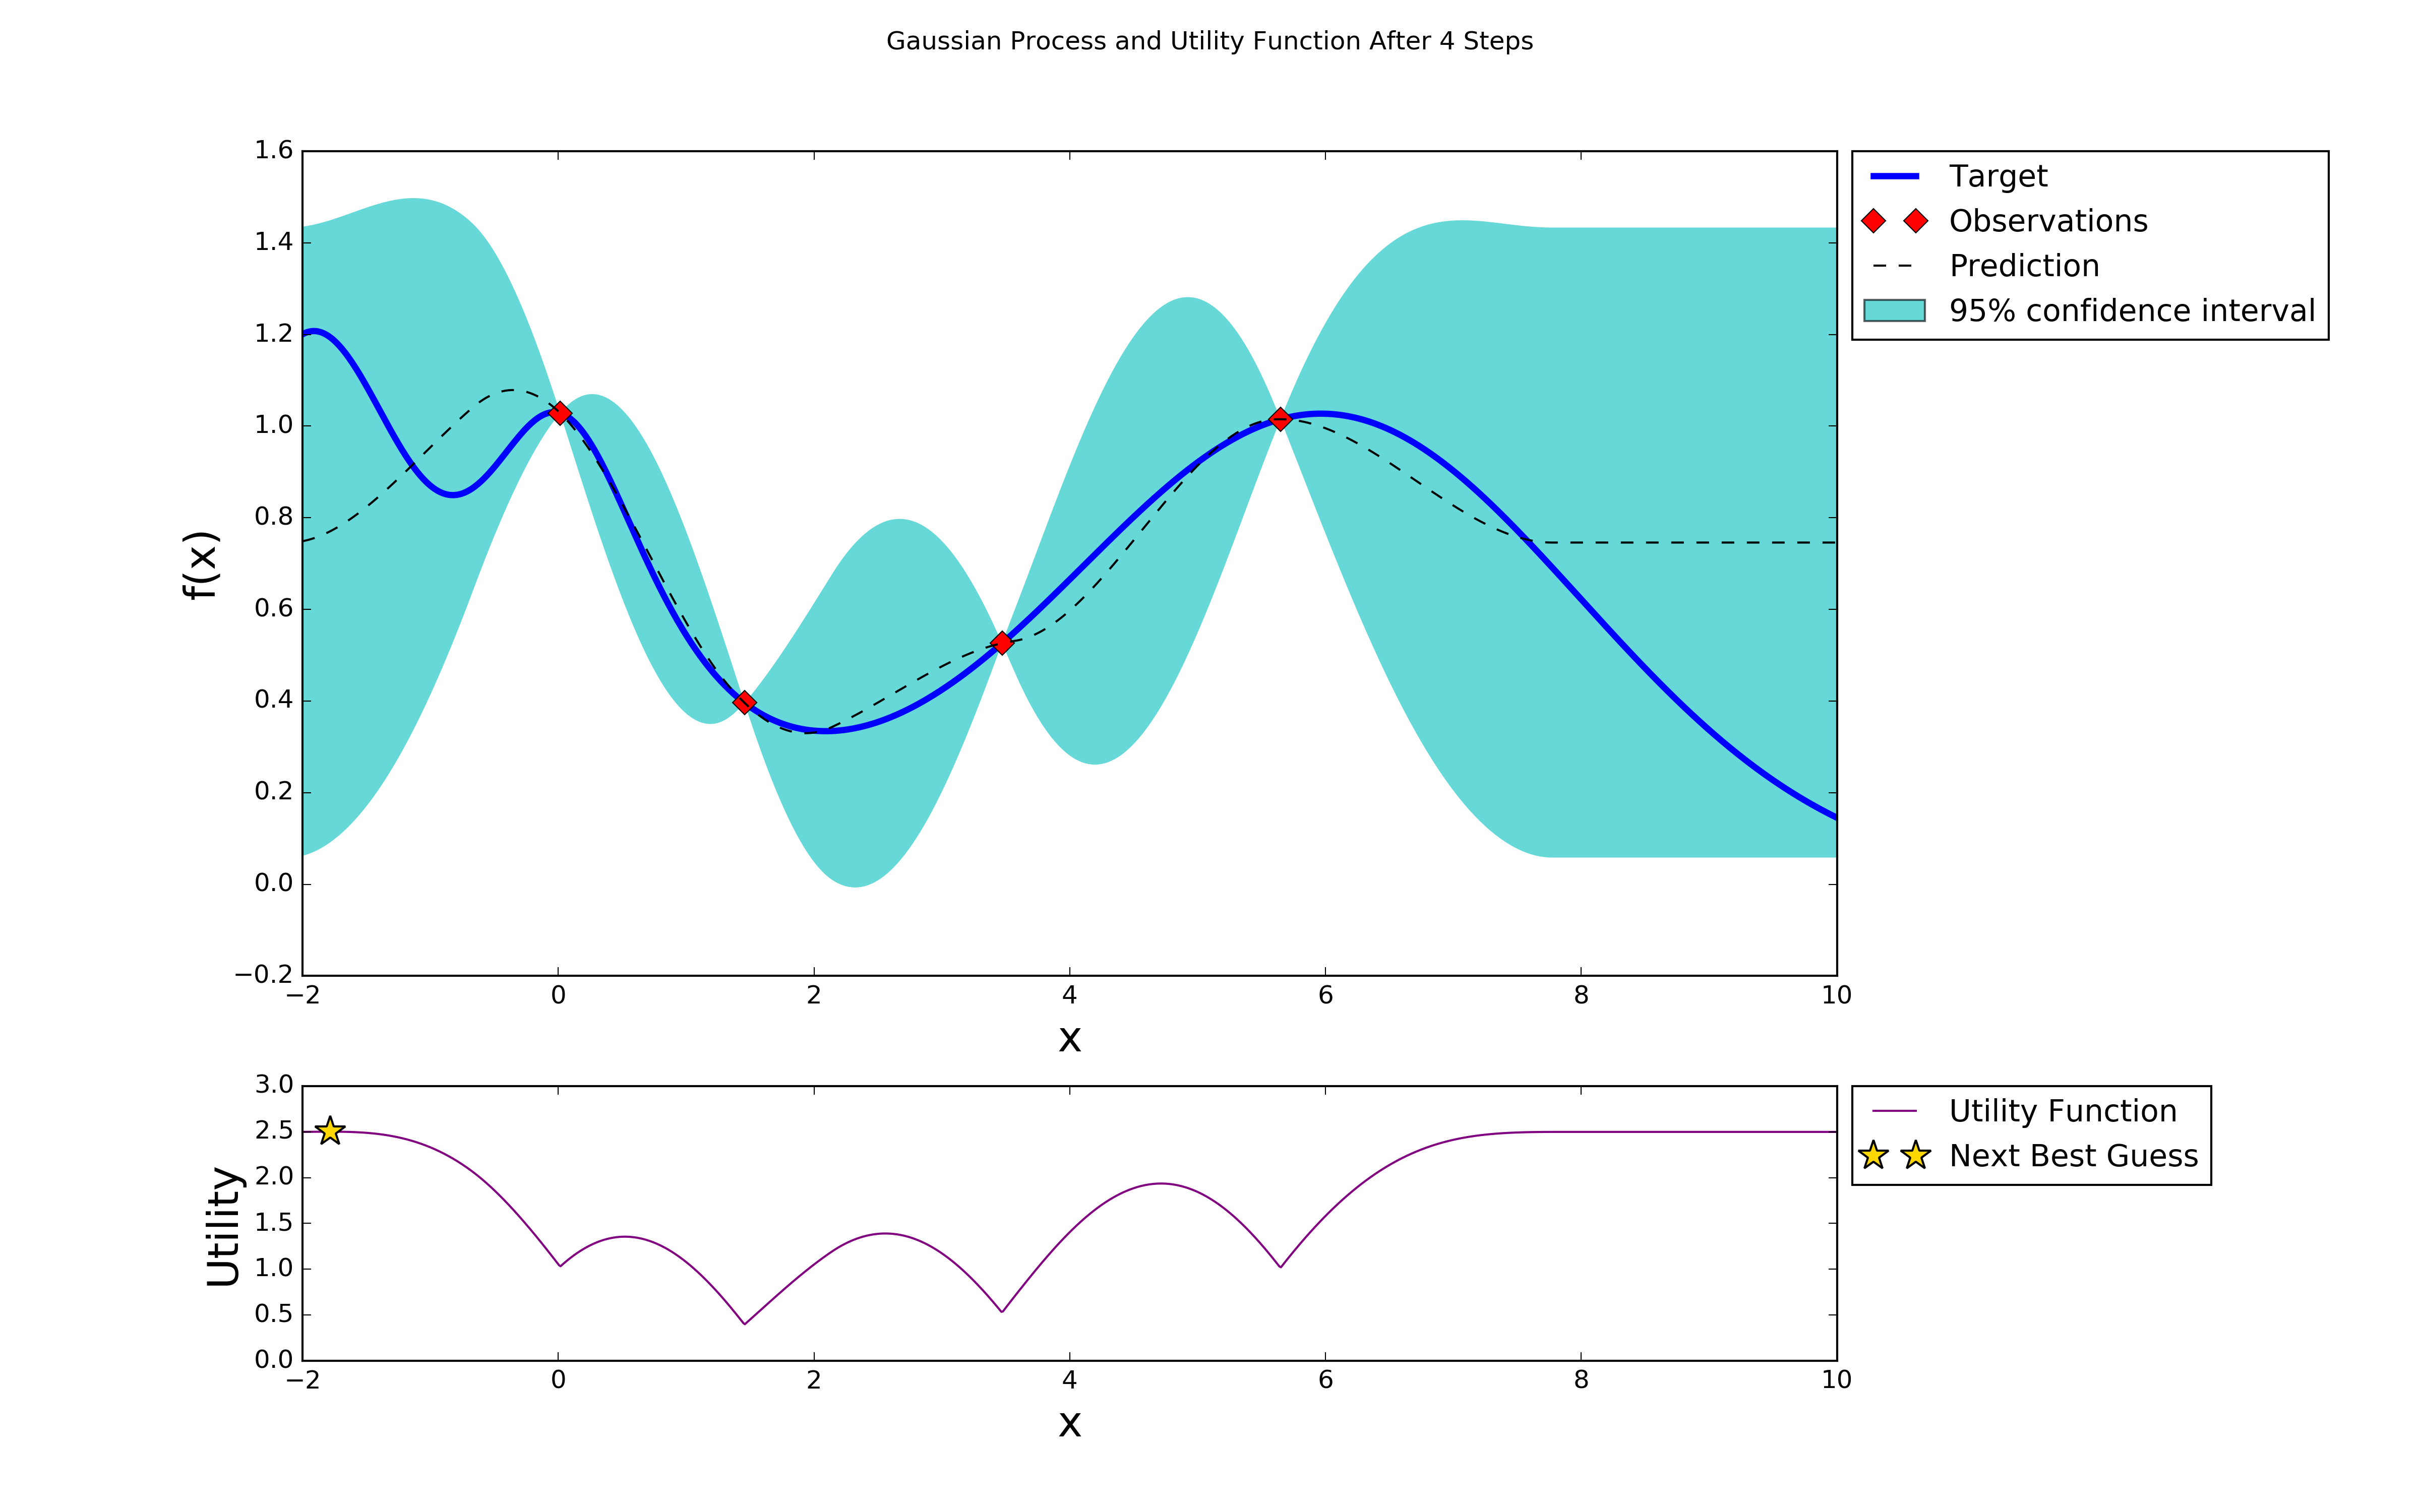
\includegraphics[width=1\textwidth]{figures/BO.png}
	\vspace{-2em}
	\caption{Example of an objective function and surrogate function. After probing observations from the objective functions the surrogate function is update to form the posterior. Uncertainty is low near observations.}
	\label{fig:bayesian-optimization}
\end{figure*}

\subsection{Kernel function}
The kernel is a function for the GP, which determines the smoothness of samples drawn from it. The choice of kernel is crucial in the process of finding the right surrogate function, to fit the objective function. Many kernels have been proposed, where one of the most used is the squared exponential function \citet{brochu2010tutorial}. The function however tends to smooth the surrogate function to much, to be applicable in real world problems. The kernel function used in this method will therefor be Matérn$\frac{5}{2}$, as proposed by \citet{snoek2012practical}.

\subsection{Acquisition function}
When Bayesian optimization builds its model of the objective function, it iteratively choses inputs to sample outputs from the objective function. The choice of which inputs to sample from is determined by the \emph{acquisition function} (AF), which determines utility of sampling from a given input. Different acquisition functions yield different measures to make this decision. One measure is the \emph{Probability of Improvement} (PI) which given a candidate input computes the probability of improving the current best result. \todo{explain with figure} Another approach is to consider the \emph{expected improvement} (EI) which not only takes into account the probability of improvement, but also the uncertainty e.g. the variance of the Gaussian distribution of the surrogate at the given input.
EI balances the trade-off between exploitation and exploring, and is therefor a well used acquisition function \citet{brochu2010tutorial}. EI(x) is the function which gives the expected improvement of choosing parameters x, and is defines as:

\begin{equation}
\label{eq:expected-improvement}
EI(x) =
\begin{cases}
   (K + L & \text{ if } \sigma(x) > 0\\
   0 	  & \text{ if } \sigma(x) = 0
\end{cases}
\end{equation}
where $K = (\mu(x) - f(x^+))\Phi(Z)$ \\and $L = \sigma(x)\phi(Z)$ .
$\mu$ and $\sigma$ are the mean and variance of the posterior distribution of the surrogate function, respectively. $Z$ is defined as:

\begin{equation}
\label{eq:expect-z}
Z =
\begin{cases}
\frac{\mu(x) - f(x^+)}{\sigma(x)} & \text{ if } \sigma(x) > 0\\
0 								  & \text{ if } \sigma(x) = 0
\end{cases}
\end{equation}
$\phi$ and $\Phi$ denote the \emph{probability density function} (PDF) and \emph{cumulative distribution function} (CDF) of the standard normal distribution.
The function for EI can then be used to probe the surrogate function with different parameter settings x, from where a new candidate point can be found to probe the objective function. The new candidate will be the parameter setting with the highest expected improvement.  


%- Combining posterior and refit the GP
